\documentclass[aspectratio=169, 8 pt]{beamer}
\usepackage{pdfpages}
\usepackage{amsmath,amsthm,amssymb}
\usepackage{tikz}
\usepackage{pstricks}
\usepackage{ragged2e}
\usepackage{mathrsfs}
\usepackage{microtype}
\usepackage{bbm}
\usepackage{graphicx, wrapfig, subcaption, setspace, booktabs}
\usepackage{tabularx}
\usepackage{listings}
\usepackage{xcolor}
\usepackage{longtable}
%\usepackage{titlesec}
\usepackage{url, lipsum}
\usepackage{hyperref,bookmark}
\usepackage[T1]{fontenc}
\usepackage{amssymb}
\usepackage{tabularx}
\usepackage{listings}
\usepackage{xcolor}
\usepackage{longtable}
\usepackage{setspace}
\usepackage{float}
\usepackage{multirow}
\usepackage{tabularx}
\usepackage[at]{easylist}% easy lists with @ starting each item
\usepackage{algorithmic}
\usepackage{graphicx}
\usepackage{textcomp}
\usepackage{amsmath}
\usepackage[sc]{mathpazo}
\usepackage{datetime}
\usepackage{graphicx, wrapfig, subcaption, setspace, booktabs}
\usepackage[T1]{fontenc}
\usepackage{fourier}
\usepackage{url, lipsum}
\usepackage{hyperref,bookmark}
\usepackage[T1]{fontenc}
\usepackage{amssymb}
\usepackage{makecell, multirow, tabularx}
\usepackage{listings}
\usepackage[ruled,linesnumbered]{algorithm2e}

\usetheme{Pittsburgh}
\ifdefined\ishandout
\usecolortheme{seagull}
\else
\usecolortheme{scottybear}
\fi

\usefonttheme{serif}
\hypersetup{colorlinks,linkcolor=,urlcolor=links}

% Theorem Styles

\theoremstyle{theorem}
\newtheorem{thm}{Theorem}
\newtheorem{lm}{Lemma}
\newtheorem{ex}{Example}
\newtheorem{exs}{Examples}

\theoremstyle{definition}
\newtheorem{defn}{Definition}
\newtheorem{notation}{Notation}

\theoremstyle{remark}
\newtheorem*{remark}{Remark}

% Commands

\DeclareMathOperator{\diam}{diam}
\DeclareMathOperator{\id}{id}

\newcommand{\8}{\infty}
\newcommand{\A}{\mathscr{A}}
\newcommand{\C}{\mathbb{C}}
\newcommand{\N}{\mathbb{N}}
\newcommand{\Q}{\mathbb{Q}}
\newcommand{\R}{\mathbb{R}}
\newcommand{\Z}{\mathbb{Z}}
\newcommand{\iunit}{\mathbbm{i}}

\newcommand{\dif}{\mathrm{d}}
\newcommand{\diff}{\,\mathrm{d}}
\newcommand{\Dim}[1]{\dim_{\mathrm{#1}}}
\newcommand{\st}{\,|\,}
\newcommand{\ST}{\,\middle|\,}
\newcommand{\Poles}{\mathscr{P}}
\renewcommand\vec[1]{\boldsymbol{#1}}
\newcommand\Union{\mathop{\bigcup}}
\newcommand\Intersect{\mathop{\bigcap}}
\newcommand\union{\mathrel{\cup}}
\newcommand\intersect{\mathrel{\cap}}

\newgray{darkgrey}{.25}
\newgray{grey}{.5}
\newgray{lightgrey}{.75}
\newgray{vlightgrey}{.9}

\newcommand{\secslide}[2]{
	\section[#1]{#2}
		\begin{frame}
			\begin{center}
				\ifdefined\ishandout
					\textbf{\Huge\secname}
				\else
					\textcolor{structure}{\textbf{\Huge\secname}}
				\fi
			\end{center}
		\end{frame}
}

\renewcommand{\baselinestretch}{1.1}


\title[]{CO\textsubscript{2} and Cost Impact Analysis of a Microgrid  with Electric Vehicle Charging Infrastructure: a Case Study in Southern California}
\author{Luis Fernando Enriquez-Contreras, Matthew Barth, Sadrul Ula}
\institute[]{Department of Electrical  and Computer Engineering \\ College of Engineering, Center for Environmental Research \& Technology \\ University of California, Riverside \\ Riverside, United States of America \\ lenri001@ucr.edu, barth@ece.ucr.edu, sula@cert.ucr.edu}
\date{September 27, 2024}


\definecolor{codegreen}{rgb}{0,0.6,0}
\definecolor{codegray}{rgb}{0.5,0.5,0.5}
\definecolor{codepurple}{rgb}{0.58,0,0.82}
\definecolor{backcolour}{rgb}{0.95,0.95,0.92}

\lstdefinestyle{mystyle}{
	backgroundcolor=\color{backcolour},   
	commentstyle=\color{codegreen},
	keywordstyle=\color{magenta},
	numberstyle=\tiny\color{codegray},
	stringstyle=\color{codepurple},
	basicstyle=\ttfamily\footnotesize,
	breakatwhitespace=false,         
	breaklines=true,                 
	captionpos=b,                    
	keepspaces=true,                 
	numbers=left,                    
	numbersep=5pt,                  
	showspaces=false,                
	showstringspaces=false,
	showtabs=false,                  
	tabsize=2
}

\lstset{style=mystyle}
\setbeamertemplate{caption}[numbered]
\begin{document}
	
	\usebackgroundtemplate{
		\tikz[overlay,remember picture] \node[opacity=0.04, at=(current page.center), yshift=-1.1in, xshift=1.75in] {
			
\includegraphics[height=3in]{aux/ucr_seal_black.eps}};
	}
	
	% ----------------------------------------------------------------------
	% TITLE SLIDE ----------------------------------------------------------
	% ----------------------------------------------------------------------
	
	\begin{frame}[plain] 
		\titlepage
		
%		\ifdefined\ishandout
%		\newcommand{\LOGO}{aux/ucr_logo_grey.eps}
%		\else
%		\newcommand{\LOGO}{aux/ucr_logo_cmyk.eps}
%		\fi
		
		\begin{tikzpicture}[remember picture,overlay]
			\node[anchor=south west,yshift=6pt,xshift=8pt] at (current page.south west) {
\includegraphics[height=1.2cm]{aux/CECERT_logo_crop.pdf}};
		\end{tikzpicture}
		
		\begin{tikzpicture}[remember picture,overlay]
			\node[anchor=south east,yshift=1pt,xshift=-6pt] at (current page.south east) {
\includegraphics[height=2cm]{aux/itsc_logo.png}};
		\end{tikzpicture}
	\end{frame}
	
	% ----------------------------------------------------------------------
	% OUTLINE --------------------------------------------------------------
	% ----------------------------------------------------------------------
	
	\begin{frame}{Outline}
		\vfill
		\tableofcontents
		\vfill
	\end{frame}
	
	\section{Introduction}
	
	\begin{frame}
		\frametitle{Abstract}	
		\begin{itemize} \LARGE
			\item This paper examines the effectiveness of transportation-based microgrid configurations in reducing CO\textsubscript{2} emissions and electricity costs within an Intelligent Transportation System (ITS)
			\item A case study at the University of California, Riverside (UCR) using CAISO CO\textsubscript{2} emission data shows that a load-following microgrid strategy can reduce CO\textsubscript{2} emissions by 67\%–84\% and save approximately \$24,000 annually, even with daily EV charging
			\item Battery sizing is crucial, as doubling capacity may lead to diminishing returns in cost and emission reductions, highlighting the need for optimal battery capacity
			\item The study finds Level 2 chargers have minimal impact on building demand, while a single Level 3 DC fast charger significantly increases demand, requiring more solar and battery storage for cost reduction
%			\item The research emphasizes balancing cost and environmental impact through strategic microgrid design and battery optimization
		\end{itemize}
		
%		\begin{itemize} \LARGE
%			\item This paper presents a case study at the University of California, Riverside (UCR) that evaluates the effectiveness of different transportation-based microgrid configurations in reducing both carbon dioxide (CO\textsubscript{2}) emissions and electricity costs
%			\item Electric costs were also compared to determine the financial savings potential for the consumer
%			\item The results demonstrate that a peak-shaving transportation-microgrid strategy can effectively reduce CO\textsubscript{2} emissions in the range of 24\% to 38\% and costs from \$27,000 to \$29,000 per year
%			\item  Careful consideration should be given to battery sizing, as peak-shaving has diminishing returns
%		\end{itemize}
\end{frame}
%	
	\begin{frame}
		\frametitle{Purpose and Contributions}
		\begin{itemize} \LARGE
			\item This research is crucial for advancing intelligent transportation systems by addressing the economic needs of EV charging infrastructure owners and optimizing configurations to benefit both EV owners and the environment.
			\item The paper investigates the impacts of Level 2 and Level 3 charging infrastructure on microgrid behavior, electricity costs, and CO\textsubscript{2} emissions in Southern California.
			\item Simulations are conducted using OpenModelica, a dynamic modeling and simulation environment.
			\item The study uses a higher time resolution, capturing CO\textsubscript{2} emissions data every 15 minutes.
			\item This approach distinguishes the research from previous studies by providing more detailed insights into emissions and cost impacts.
		\end{itemize}
		
%		\begin{itemize} \LARGE
%			\item This research holds significant implications for the advancement of intelligent transportation systems, as it aims to address the economic needs of EV charging infrastructure owners and determine the optimal configuration that benefits both EV owners and the environment by minimizing greenhouse gas emissions
%			\item This paper delves into the impacts of transportation-microgrids equipped with Level 2 and Level 3 charging on the behavior of microgrids, associated electricity costs, and CO\textsubscript{2} emissions within the context of southern California
%			\item The simulations are conducted using OpenModelica, a dynamic modeling and simulation environment
%			\item This study distinguishes itself from previous research in many ways, including employing a higher time resolution for calculating CO\textsubscript{2} emissions that is measured every 15 minutes
%		\end{itemize}
	\end{frame}
	
	\section{Methodology}
	
	\begin{frame}
		\frametitle{Microgrid Setup in OpenModelica}
		\begin{figure}
			\centering
			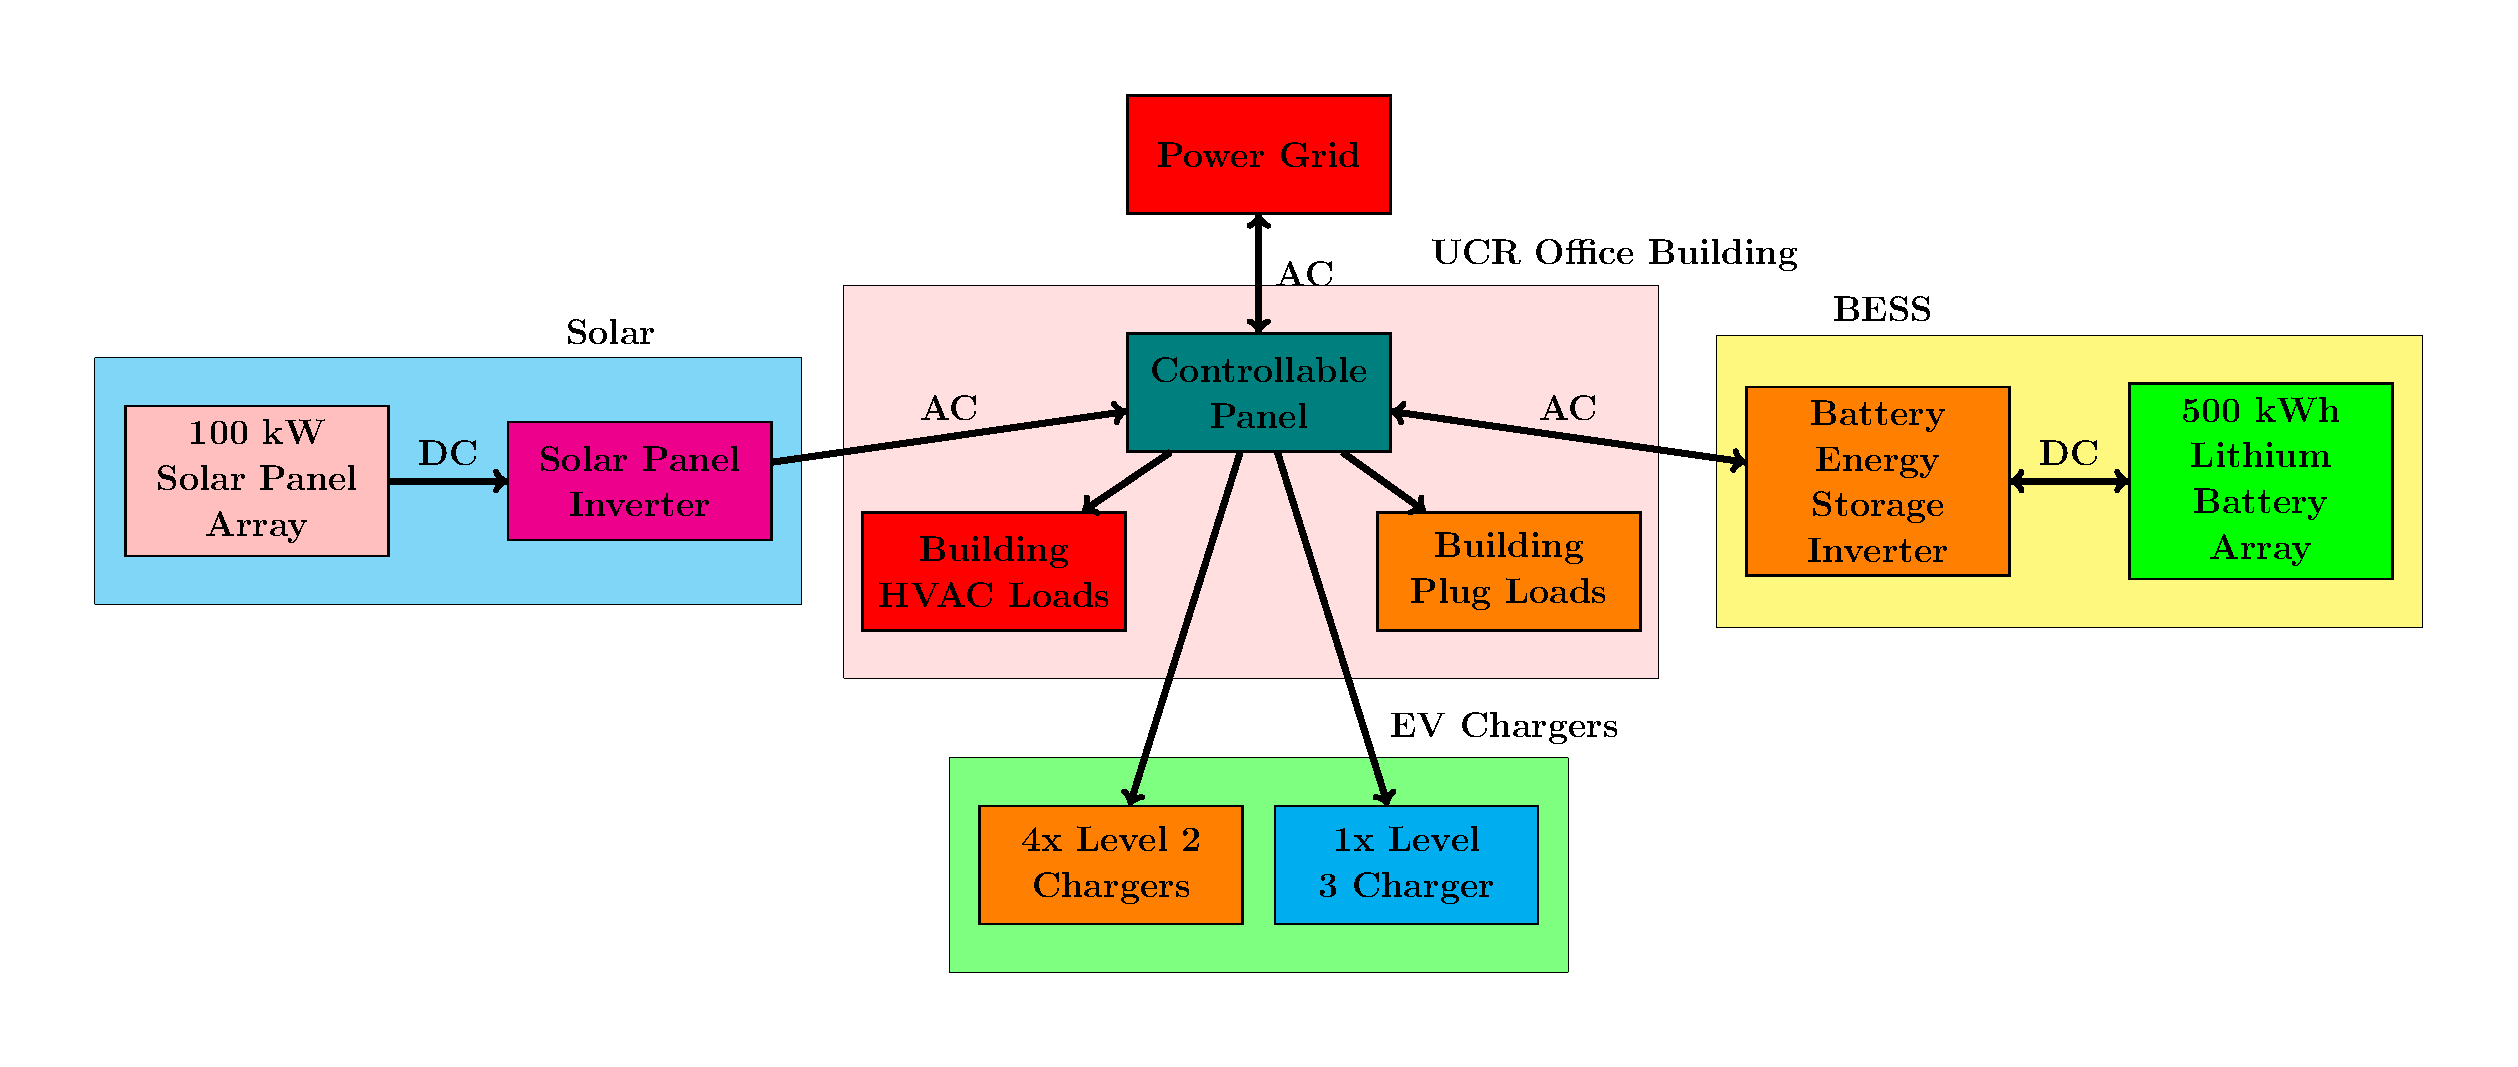
\includegraphics[width=0.88\linewidth]{Fig/power_system_setup_modelica_large}
			\caption{Microgrid Architecture of our Case Study Example BESS: Battery Energy Storage System}
			\label{fig:powersystemsetupfull}
		\end{figure}
	\end{frame}
	
	\begin{frame}
		\frametitle{EV Charger Loads}
		Our model incorporates transportation loads through EV charging infrastructure, including both real-world Level 2 chargers (as depicted in Figs. \ref{fig:l2avgdayrandpoisson1hourpdf} and \ref{fig:level2cert}) and simulated Level 3 chargers modeled using a Poisson distribution.
		\begin{columns}
			\begin{column}{0.5\linewidth}
				\begin{block}{}
					\begin{figure}
						\centering
						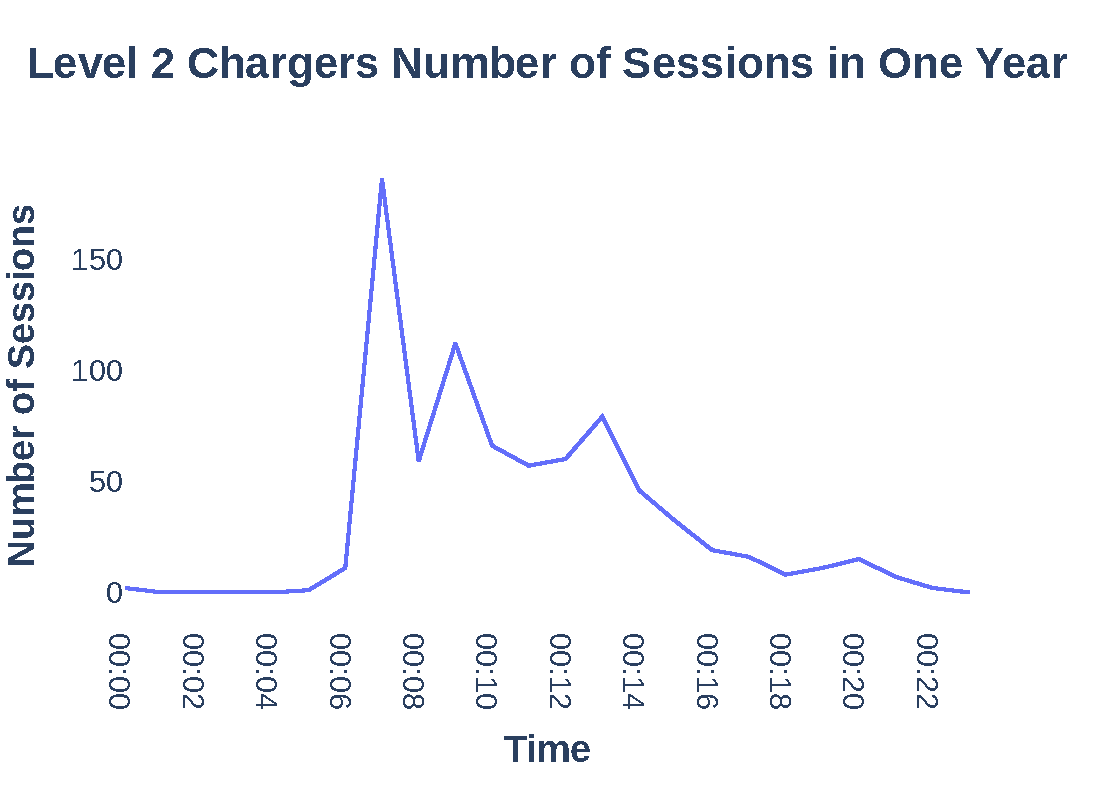
\includegraphics[width=0.9\linewidth]{Fig/Option_3/l2_avg_day_rand_poisson_1_hour_real.pdf}
						\caption{\footnotesize Level 2 EV Charger Probability Density Function  Created  by Using Actual Charging Data Obtained from a SCADA System}
						\label{fig:l2avgdayrandpoisson1hourpdf}
					\end{figure}
				\end{block}
			\end{column}
			\begin{column}{0.5\linewidth}
				\begin{block}{}
					\begin{figure}
						\centering
						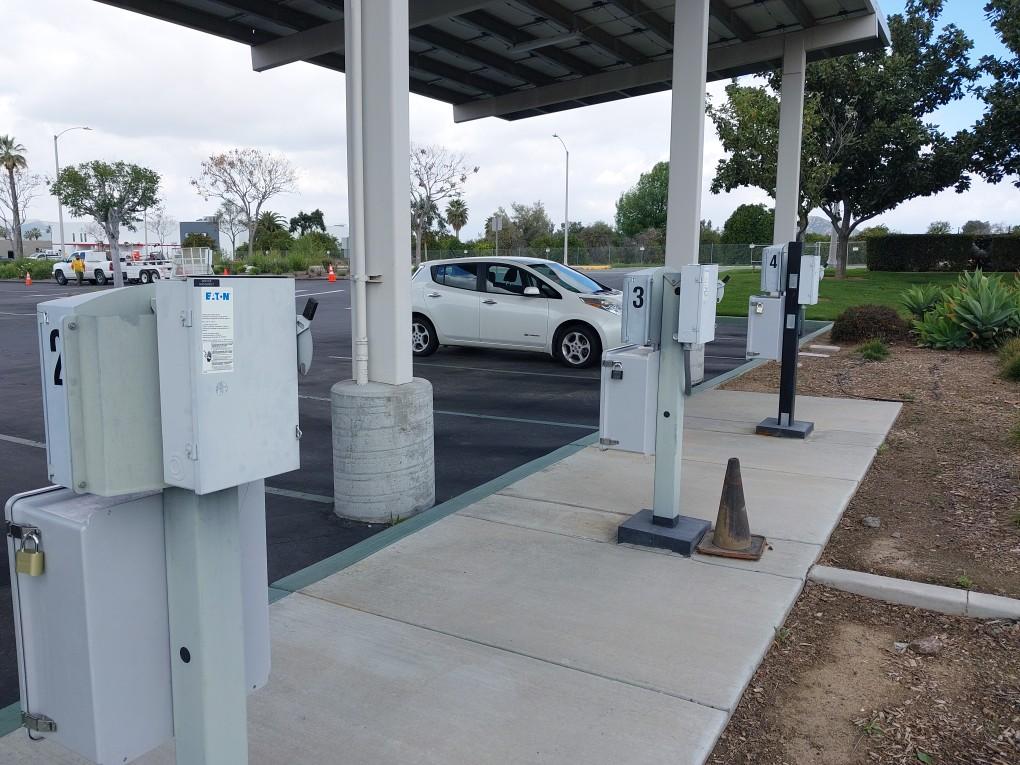
\includegraphics[width=0.9\linewidth]{Fig/Option_3/level_2_cert}
						\caption{Level 2 Charging Setup}
						\label{fig:level2cert}
					\end{figure}
				\end{block}
			\end{column}
		\end{columns}
	\end{frame}
	
	\section{Results}	
	
	\begin{frame}
		\frametitle{Results}
		\begin{itemize}
			\item The charging setup is modified in OpenModelica for different layouts and scenarios
			\item The scenarios are described in Table \ref{tab:scenarios}
		\end{itemize}
		
		\begin{table}
			\caption{Simulated Scenarios of the example UCR Microgrid under Different Battery Sizes and EV Charging Demands}
			\large
			\begin{tabularx}{\linewidth}{l | l}
\toprule
 Scenario &  \\
\midrule
		1  & Standard Building with no EV Chargers\\
        2 & Standard Building with Level 2 Charging\\
        3 & Standard Building with Level 2 and Level 3 Charging \\
        4 &  Microgrid Building with 100 kW Solar, 500 kWh BESS, and No EV Charging\\
        5 & Microgrid Building with 100 kW Solar, 500 kWh BESS,  and Level 2 Charging\\
        6 & Microgrid Building with 100 kW Solar, 500 kWh BESS, Level 2, and Level 3 Charging\\
        7 & Microgrid Building with 100 kW Solar, 1 MWh BESS, and Level 2 Charging\\
        8 & Microgrid Building with 100 kW Solar, 2 MWh BESS, Level 2, and Level 3 Charging\\
\bottomrule
\end{tabularx}

			\normalsize
			\label{tab:scenarios}
		\end{table}
	\end{frame}
	
	\begin{frame}
		\frametitle{Results}
		\begin{table}
			\caption{Microgrid Utility Prices and CO\textsubscript{2} Emissions Output under Different Battery Sizes and EV Charging Demands}
			\centering
				\large
				\begin{tabular}{rrrrr}
\toprule
 Scenario &  Demand Charges (\$) &  Energy Charges (\$) &  Total Cost (\$) &  Emissions \\
\midrule
        1 &                6616 &               22736 &           29352 &         34 \\
        2 &                8196 &               24607 &           32803 &         37 \\
        3 &                3887 &                1556 &            5443 &          5 \\
        4 &               11744 &                5841 &           17585 &         23 \\
        5 &                5133 &                3256 &            8389 &          7 \\
        6 &               11329 &                8091 &           19420 &         14 \\
        7 &                5022 &                3396 &            8418 &          7 \\
        8 &               11400 &                8075 &           19475 &         14 \\
\bottomrule
\end{tabular}

			\normalsize
			\label{tab:emissions}
		\end{table}	
	\end{frame}
	
	\begin{frame}
		\frametitle{Results}
		\begin{figure}
			\centering
			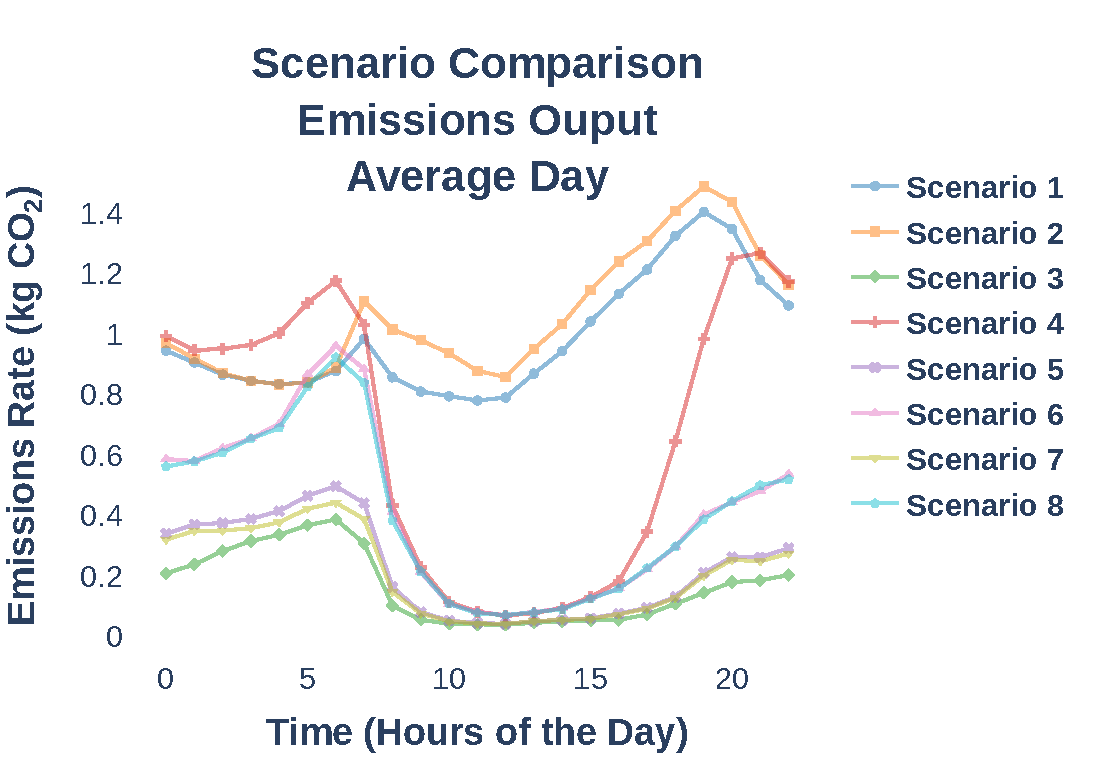
\includegraphics[width=0.73\textwidth]{Fig/Option_3/emissions_scenario_comparison_run_3_large_font.pdf}
			\caption{\footnotesize  CO\textsubscript{2} Emissions Outputs Averages During Times of Day, using a microgrid setup}
			\label{fig:emissionsscenariocomparison}
		\end{figure}
	\end{frame}
	
%	\begin{frame}
%		\frametitle{Results}
%		\begin{columns}
%			\begin{column}{0.5\linewidth}
%				\begin{block}{}
%					\begin{figure}
%						\centering
%						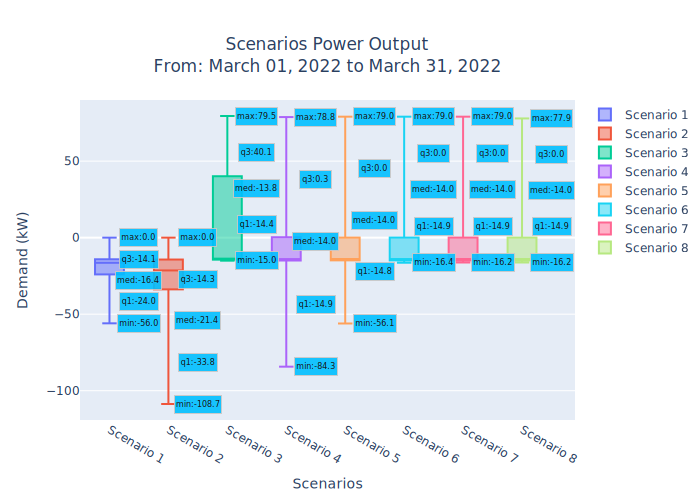
\includegraphics[width=1\linewidth]{Fig/Option_3/0_Scn_Output_Run_3_Mar_01_2022_to_Mar_31_2022}
%						\caption{\footnotesize  Power measured from the meter for March}
%						\label{fig:0scnoutputrun2mar012022tomar312022}
%					\end{figure}
%				\end{block}
%			\end{column}
%			\begin{column}{0.5\linewidth}
%				\begin{block}{}
%					\begin{figure}
%						\centering
%						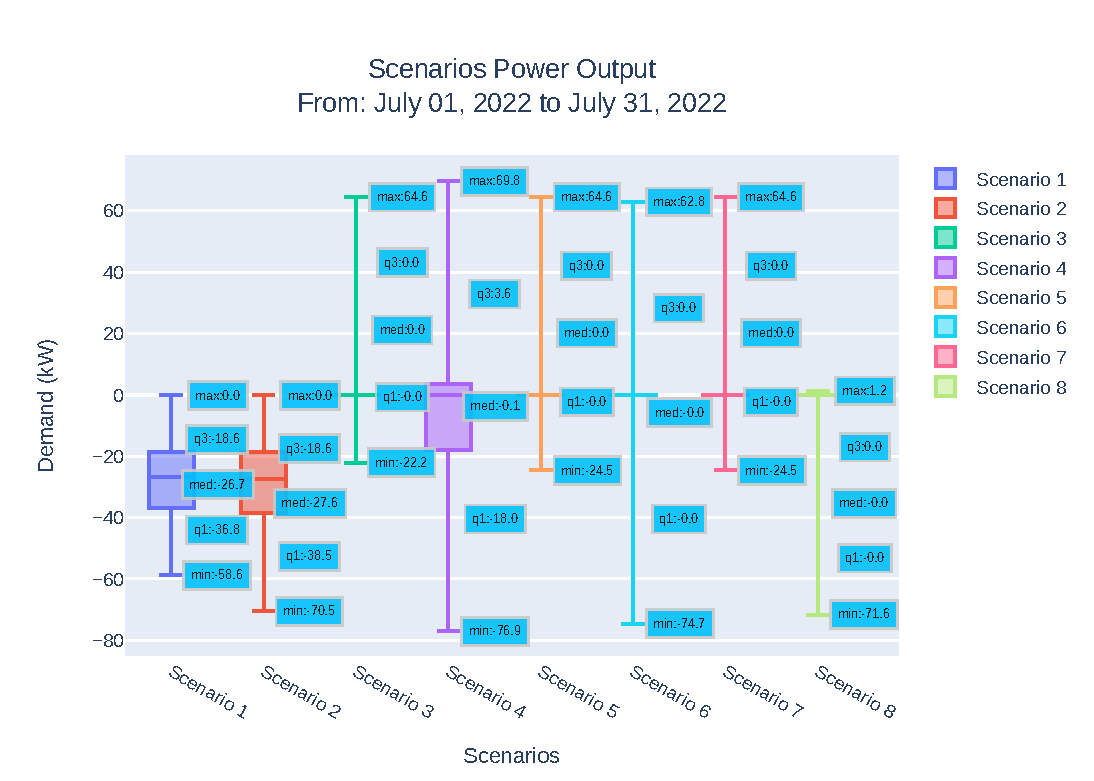
\includegraphics[width=1\linewidth]{Fig/Option_3/4_Scn_Output_Run_3_Jul_01_2022_to_Jul_31_2022}
%						\caption{\footnotesize  Power measured from the meter for July}
%						\label{fig:4scnoutputrun2jul012022tojul312022}
%					\end{figure}
%				\end{block}
%			\end{column}
%		\end{columns}
%	\end{frame}
	
	\begin{frame}
	\frametitle{Results}
	\begin{columns}
		\begin{column}{0.5\linewidth}
			\begin{block}{}
				\begin{figure}
					\centering
					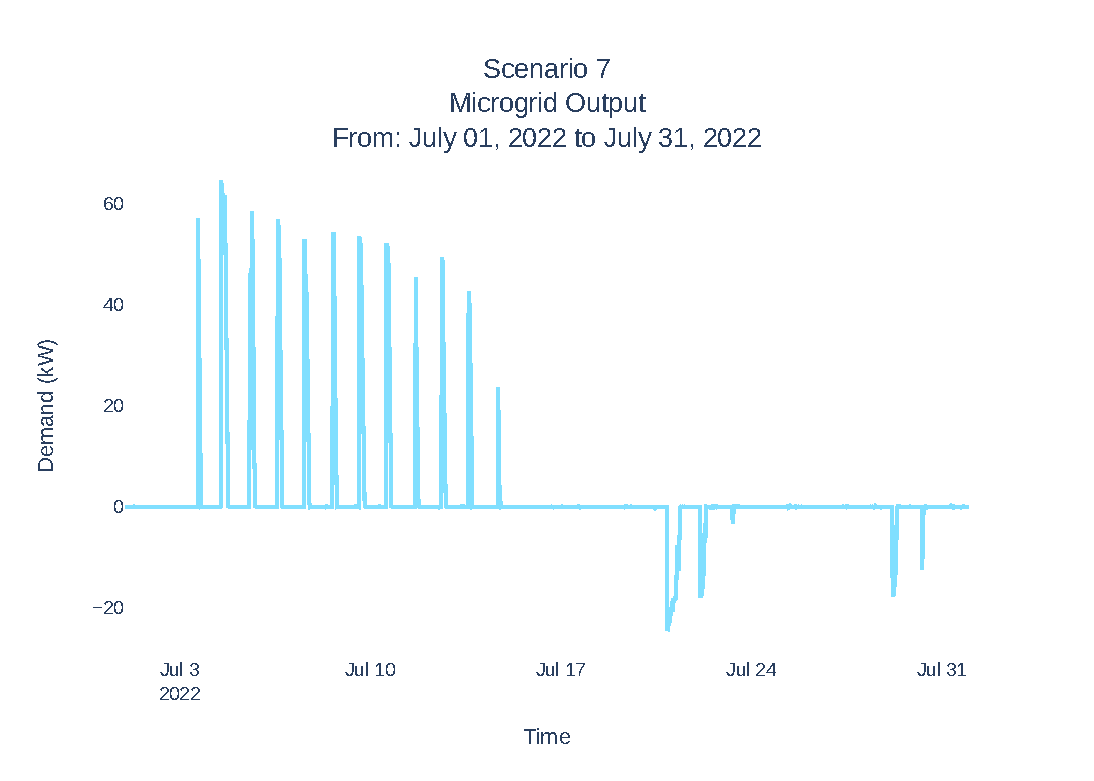
\includegraphics[width=\linewidth]{Fig/Option_3/4_Scenario_7_Run_3_Mg_Output_Jul_01_2022_to_Jul_31_2022.pdf}
					\caption{\footnotesize Load Following Failures after Battery Depletion (Level 2 Charging, 1 MWh BESS)}
					\label{fig:scenario3peakshaving}
				\end{figure}
			\end{block}
		\end{column}
		\begin{column}{0.5\linewidth}
			\begin{block}{}
				\begin{figure}
					\centering
					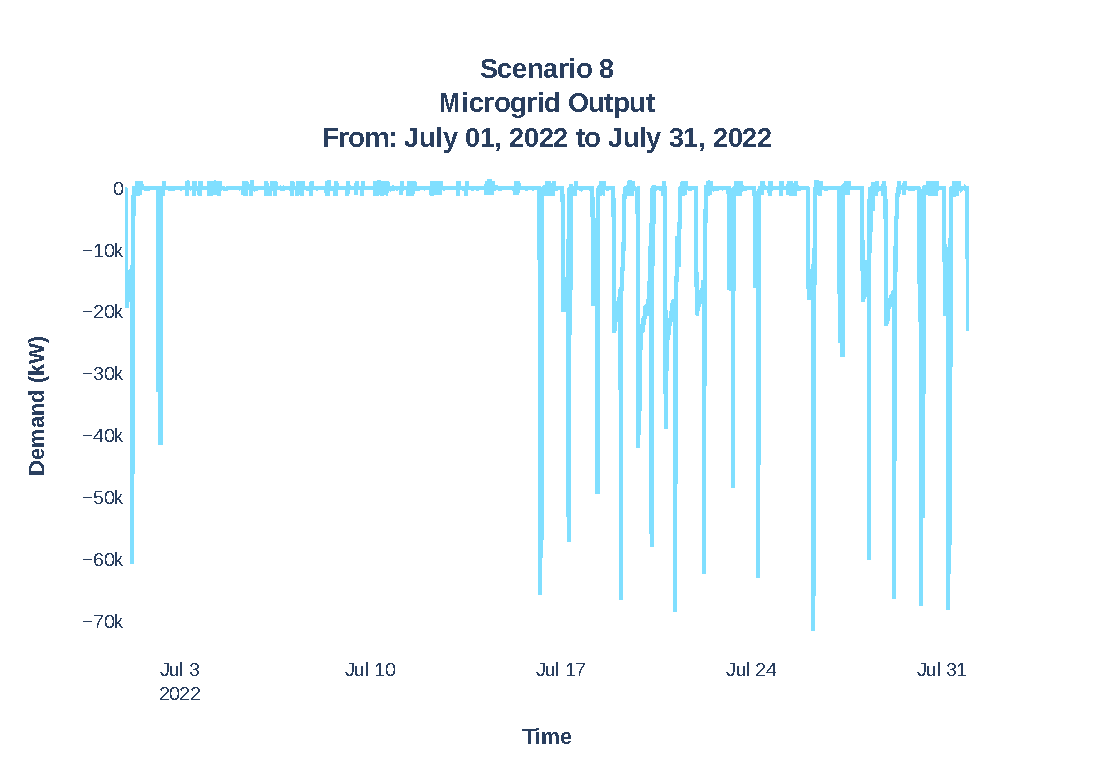
\includegraphics[width=\linewidth]{Fig/Option_3/4_Scenario_8_Run_3_Mg_Output_Jul_01_2022_to_Jul_31_2022.pdf}
					\caption{\footnotesize Load Following Failures after Battery Depletion (Level 2 and Level 3 Charging, 1 MWh BESS)}
					\label{fig:scenario4peakshaving}
				\end{figure}
			\end{block}
		\end{column}
	\end{columns}
\end{frame}
	
	\section{Conclusions and Future Work}		
	
	\begin{frame}
		\frametitle{Conclusions}
		\begin{itemize} \Large
			\item Transportation-microgrids offer significant economic and environmental benefits
			\begin{itemize} \large
				\item Annual savings for load-following transportation microgrids are approximately \$23,000 to \$24,000, despite the additional demand from EV chargers.
				\item Cost of demand and energy savings trends are similar, with savings of \$3,000 and \$21,000 respectively.
				\item Load-following microgrids can reduce CO\textsubscript{2} emissions by 67\% to 85\%, equating to about 30 tons of CO\textsubscript{2} reduction.
			\end{itemize}
			\item Increased battery capacity does not guarantee improved performance
			\begin{itemize} \large
				\item Increased capacity improves performance but not proportionally to the cost
				\item Large capacity needed for challenging situations may not be cost-effective 
			\end{itemize}
			\item Key considerations for effective microgrid implementation and clean energy integration
			\begin{itemize} \large
				\item Incentives exist to integrate additional clean energy sources (solar and wind), particularly when incorporating Level 3 fast chargers
				\item Level 2 chargers have a minimal impact on office building energy demands
				\item Effective microgrid planning requires a balance of clean energy generation, energy storage, and load management
			\end{itemize}
		\end{itemize}
	\end{frame}
	\begin{frame}
		\frametitle{Future Work}
		\begin{itemize} \LARGE
			\item Explore advanced control strategies to optimize electric costs and CO\textsubscript{2} emissions for microgrids energy management
			\item Investigate electric vehicle load allocation during high peak times
			\item Minimize power drawn from the grid during periods of high CO\textsubscript{2} emissions.
			\item Assess the effects of the new net energy metering policy in California on the value of the Battery Energy Storage System (BESS).
			\item Analyze the impact of different time-of-use (TOU) rates in California on electric costs and CO\textsubscript{2} emissions.
		\end{itemize}
	\end{frame}
	
	\begin{frame}
		\frametitle{\null}
		\centering
		\Huge
		Questions?
	\end{frame}
	
	\begin{frame}
		\frametitle{\null}
		\centering
		\Huge
		Thank You
	\end{frame}
\end{document}
